\documentclass[class=article, crop=false]{standalone}
\usepackage{graphicx}
\graphicspath{{../Figures}}

\begin{document}

\section{Case results}
One case was tested in which the ROV and USV are initialized at the desired point to hold with a given seastate. There are two variables which have been tested: the length of the wire (and thus the starting depth of the ROV) and the waveheight. Specifically, the ROV's height was tested at 0m (analogous to being stowed), 50m and 100m. 0m was chosen as a baseline, showing the USV's performance when not affected by the drag of the ROV. From the plans for the project at the time of writing, the planned maximum operating depth is 100m, making this a natural second datapoint. 50m was chosen as a midpoint between the two for additional data collection.

Data was gathered by a data collection ROS2 node which collected, worked and plotted the data.

\begin{figure}
    \centering
    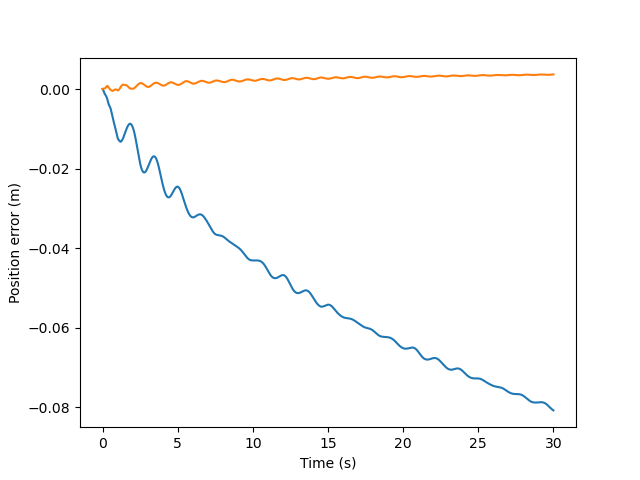
\includegraphics{scenario1/rov-0m/0.0m/usv_pos_error_uncontrolled}
    \caption{Position of the USV uncontrolled}

\end{figure}

\subsection{}

\section{Simulation results}
As mentioned in previous chapters, the simulation was a continued work basedon a specialization project which was undertaken in the fall semester of 2024. The goal of the simulation was to simulate the physical situation to allow for tuning and development of the controller. As such, using the commercially available simulation framework AGX Dynamics, developed by Algoryx AB was seen as reasonable.

AGX Dynamics is used as a simulation framework for both machine-in-the-loop systems as well as for simulation of dynamic systems including wires, granulates and hydrodynamic/aerodynamic situations. The reasoning has been that if it's good enough for these purposes it will be good enough for this project.

\subsection{Validation}
Validation of the simulator was primarily performed in the specialization project. There it was done as both an imperical measurement as well as a more general measurement. The specialization project found that the simulator performs as expected.

As a summary of the validation, the tension experienced by the tether between the ROV and the USV was both calculated using manual methods and simulated. The calculations and simulations were performed at 6 different speeds, between 0m/s and 5m/s in 1m/s increments. The ROV was observed in the simulations to drag behind the USV, since the USV is the powered part in this validation and the ROV is only hanging behind as a passive part. As the angle of the tether changes, the cross-sectional area of the ROV as well as the drag coefficient changes. To account for this, the calculated drag was calculated at two separate drag coefficients, one for a flat-facing cuboid and one for an edge-facing cuboid, respectively chosen from tables as 2.05 and 1.05. The forward facing area was assumed in calculations to be constant, however this is an obvious simplification and source of error.

The tension calculated on the wire was compared to the tension provided by the simulator, and was found to be within an acceptable range of error. The deviation between calculation and simulation was found to be between 3\% and 55\%, which considering the severe simplifications assumed makes the results of the simulation seem valid. Additionally, as could be expected, the deviation between calculation and simulation changes as the speed, and thus the drag coefficient and forward facing area, changes. At low speeds, the lower drag coefficient provides more accurate results, while at higher speeds the higher drag coefficient provides more accurate results. This is likely an effect of the forward facing area changing significantly, but is consistent with the expectation looking at the simulation, that the drag increases with speed. Accounting for this change in drag with speed, the deviation can be said to be between 3\% and 20\%, which is definitely within acceptable ranges for accuracy.

All these elements are discussed further and in greater detail in section 4 of the specialization project.

\subsection{Limitations}
The simulator is currently not implemented with a winching motion available, and control for the ROV is also not implemented as it stands. ROV control has been implemented before while the controller was a part of the simulation script, but has not been reimplemented as ROS2 has been implemented in the system. These elements have been deprioritized in order to allow for the physical testing of the vessel and its control system. Ideally, the implementation of these elements will not be very time consuming, nor will they affect the greater system as is the goal of the node-based system of ROS2.

\section{Controller results}

\subsection{USV}



\section{Results of physical testing}

\end{document}
